\documentclass[a4paper]{beamer}%handout


\usepackage{listings}
\usepackage{color}
 
\definecolor{codegreen}{rgb}{0,0.6,0}
\definecolor{codegray}{rgb}{0.5,0.5,0.5}
\definecolor{codepurple}{rgb}{0.58,0,0.82}
\definecolor{backcolour}{rgb}{0.95,0.95,0.92}


%% Add Matlab code
\usepackage{mcode}
%% Add Matlab code end


%% Add watermarks
%\usepackage{draftwatermark}
%% Add watermarks end
\usepackage[utf8]{inputenc}
\usepackage{multicol}
\usepackage{url}
\usepackage{hyperref}
\hypersetup{
	colorlinks=true,
	linkcolor=cyan,          % color of internal links (change box color with linkbordercolor)
    citecolor=green,        % color of links to bibliography
    filecolor=magenta,      % color of file links
    urlcolor=cyan           % color of external links
	}

\graphicspath{{img/}}

\mode<presentation> {

%\usetheme{default}%yes % use %\frametitle in all slides recommended
%\usetheme{AnnArbor}%no
%\usetheme{Antibes} %yes %favorite
%\usetheme{Bergen} %no
%\usetheme{Berkeley} %no
%\usetheme{Berlin} %no
%\usetheme{Boadilla} %yes % good use of paper space
%\usetheme{CambridgeUS} %yes %favorite %use %\frametitle recommended
%\usetheme{Copenhagen}%yes%noframetitle
%\usetheme{Darmstadt}%no
%\usetheme{Dresden}
%\usetheme{Frankfurt}
%\usetheme{Goettingen}
%\usetheme{Hannover}
%\usetheme{Ilmenau}%no
%\usetheme{JuanLesPins}
%\usetheme{Luebeck}
%\usetheme{Madrid}
%\usetheme{Malmoe}
%\usetheme{Marburg}
%\usetheme{Montpellier}
%\usetheme{PaloAlto}
%\usetheme{Pittsburgh}%no
%\usetheme{Rochester}%no
%\usetheme{Singapore}%yees
%\usetheme{Szeged}%no
%\usetheme{Warsaw}%no

% As well as themes, the Beamer class has a number of color themes
% for any slide theme. Uncomment each of these in turn to see how it
% changes the colors of your current slide theme.

%\usecolortheme{albatross}
%\usecolortheme{beaver}
%\usecolortheme{beetle}
%\usecolortheme{crane}
\usecolortheme{dolphin}
%\usecolortheme{dove}
%\usecolortheme{fly}
%\usecolortheme{lily}
%\usecolortheme{orchid}
%\usecolortheme{rose}
%\usecolortheme{seagull}
%\usecolortheme{seahorse}
%\usecolortheme{whale}
%\usecolortheme{wolverine}

\setbeamertemplate{footline} % To remove the footer line in all slides uncomment this line
%\setbeamertemplate{footline}[page number] % To replace the footer line in all slides with a simple slide count uncomment this line

\setbeamertemplate{navigation symbols}{} % To remove the navigation symbols from the bottom of all slides uncomment this line
}

%----------------------------------------------------------------------------------------
%	NEW COMMANDS
%----------------------------------------------------------------------------------------

\newcommand{\Conv}{\mathop{\scalebox{1.5}{\raisebox{-0.2ex}{$\ast$}}}}%
%\linespread{1.3}

%----------------------------------------------------------------------------------------
%	TITLE PAGE
%----------------------------------------------------------------------------------------

\title[Introduction]{Digital Image Processing} % The short title appears at the bottom of every slide, the full title is only on the title page

\author{Prof. Tiago Vieira} % Your name
\institute[UFAL] % Your institution as it will appear on the bottom of every slide, may be shorthand to save space
{
Universidade Federal de Alagoas \\ % Your institution for the title page
\medskip
\textit{tvieira@ic.ufal.br} % Your email address
}
\date{\today} % Date, can be changed to a custom date


%------------------------------------------------

\begin{document}

%------------------------------------------------

\begin{frame}
\titlepage % Print the title page as the first slide
\end{frame}

%------------------------------------------------

\begin{frame}{Contents}
\setcounter{tocdepth}{1}
\tableofcontents
\end{frame}



%----------------------------------------------------------------------------------------
%	PRESENTATION SLIDES
%----------------------------------------------------------------------------------------

\section{Introduction}

%----------------------------------------------------------------------------------------

\subsection{What's DIP?}

%----------------------------------------------------------------------------------------

\begin{frame}{Introduction -- What's DIP?}
\begin{itemize}
\item Science mixed with art.
\item Interdisciplinary territory.
\item Stimulates scientific research, development and innovation.
\end{itemize}
\end{frame}

%----------------------------------------------------------------------------------------

%\begin{frame}
%\textit{What my friends think I do}.
%\begin{figure}
%\centering
%\includegraphics[width=.7\textwidth]{skin-detection-1.png}
%\end{figure}
%\end{frame}
%
%%----------------------------------------------------------------------------------------
%
%\begin{frame}
%\textit{What I really do}. Skin detection.
%\begin{figure}
%\centering
%\includegraphics[width=.7\textwidth]{skin-detection-2.png}
%\end{figure}
%\end{frame}

%----------------------------------------------------------------------------------------

\begin{frame}
Connected areas:
\begin{itemize}
\item Computer graphics.
\item Computer vision.
\item Robotics.
\item Remote sensing.
\end{itemize}
\end{frame}

%----------------------------------------------------------------------------------------

\begin{frame}
Desired knowledges:
\begin{itemize}
\item Mathematics.
\item Statistics.
\item Algorithms.
\item Signals and systems.
\end{itemize}
\end{frame}

%----------------------------------------------------------------------------------------

\begin{frame}
Contrast enhancement:
\begin{figure}
\centering
\includegraphics[width=\textwidth]{contrast.png}
\end{figure}
\end{frame}

%----------------------------------------------------------------------------------------

\begin{frame}
Contrast enhancement:
\begin{figure}
\centering
\includegraphics[width=\textwidth]{contrast-1.png}
\end{figure}
\end{frame}

%----------------------------------------------------------------------------------------

\begin{frame}
Contrast enhancement:
\begin{figure}
\centering
\includegraphics[width=\textwidth]{contrast-2.png}
\end{figure}
\end{frame}

%----------------------------------------------------------------------------------------

\begin{frame}
What is the magic?
\begin{itemize}
\item Understand the relation between the data and what we observe.
\item Model properly what we have and what we want.
\item Possess a good set of tools allowing us to achieve the desired result with the least computational effort.
\end{itemize}
\end{frame}

%----------------------------------------------------------------------------------------

\begin{frame}
Selective contrast enhancement.
\begin{figure}
\centering
\includegraphics[width=\textwidth]{contrast-3.png}
\end{figure}
\end{frame}

%----------------------------------------------------------------------------------------

\begin{frame}
\begin{figure}
\centering
\includegraphics[width=\textwidth]{contrast-4.png}
\end{figure}
\end{frame}

%----------------------------------------------------------------------------------------

\begin{frame}
Blurring.
\begin{figure}
\centering
\includegraphics[width=.7\textwidth]{blurring.png}
\end{figure}
\end{frame}

%----------------------------------------------------------------------------------------

\begin{frame}
Terrain labelling.
\begin{figure}
\centering
\includegraphics[width=\textwidth]{terrain.png}
\end{figure}
\end{frame}

%----------------------------------------------------------------------------------------

%\begin{frame}
%Forest tomography with SAR.
%\begin{figure}
%\centering
%\includegraphics[width=\textwidth]{forest-tomography.png}
%\end{figure}
%\end{frame}

%----------------------------------------------------------------------------------------

\begin{frame}
Boat detection.
\begin{figure}
\centering
\includegraphics[width=\textwidth]{boat-detection.png}
\end{figure}
\end{frame}

%----------------------------------------------------------------------------------------

\begin{frame}
Terrain deformation analysis.
\begin{figure}
\centering
\includegraphics[width=\textwidth]{terrain-deformation.png}
\end{figure}
\end{frame}

%----------------------------------------------------------------------------------------

\begin{frame}
\begin{columns}[T]
\begin{column}{.6\textwidth}
\begin{itemize}
\item An image:
\begin{itemize}
\item Bi-dimensional function $f(x,y)$.
\item Amplitude of $f(x,y)$ at any pair of coordinates $(x,y)$ is called \textit{intensity} or \textit{gray level}.
\end{itemize}
\item When $x$, $y$ and $f(x,y)$ are finite	the image is \textit{digital}.
\item Digital image processing = process digital images using a digital computer.
\end{itemize}
\end{column}
\begin{column}{.4\textwidth}
\begin{figure}
\includegraphics[width=.48\textwidth]{LetterA.png}
\end{figure}
\end{column}
\end{columns}
\end{frame}

%----------------------------------------------------------------------------------------

\begin{frame}
A digital image is composed by a finite number of elements, AKA:
\begin{itemize}
\item Picture elements.
\item Image elements.
\item Pels.
\item Pixels.
\end{itemize}
Paradigm:
\begin{itemize}
\item Where does IP stops and where does it stop?
\item (\textit{Narrow definition}) In IP, both input and output are images.
\end{itemize}
\end{frame}

%----------------------------------------------------------------------------------------

\begin{frame}
Another paradigm, according to processing level:
\begin{itemize}
\item Low-level:
\begin{itemize}
\item Primitive operations.
\item Noise-reduction, pre-processing steps.
\item Content enhancement.
\item Sharpening.
\end{itemize}
\item Mid-level:
\begin{itemize}
\item Segmentation.
\item Classification.
\end{itemize}
\end{itemize}
\end{frame}

%----------------------------------------------------------------------------------------

\begin{frame}
\begin{itemize}
\item High-level:
\begin{itemize}
\item Understanding.
\item Cognitive functions.
\end{itemize}
\end{itemize}
\begin{table}
\centering
\begin{tabular}{|c|c|c|}
\hline 
Processing level & Input & Output \\ 
\hline 
\hline
Low & Image & Image \\ 
\hline 
Mid & Generally image & Attribute \\ 
\hline 
High & Attribute & Significance \\ 
\hline 
\end{tabular} 
\end{table}
\begin{figure}
\includegraphics[width=.5\textwidth]{paradigm.pdf}
\end{figure}
\end{frame}

%----------------------------------------------------------------------------------------
\section{Origins}

%----------------------------------------------------------------------------------------

\begin{frame}
\frametitle{Origins - Newspaper industry}
\begin{columns}
\begin{column}{.5\textwidth}
\begin{itemize}
\item Pictures sent by submarine cable.%~\cite{1450705}.
\begin{itemize}
\item (1920) Bartlane cable (London $\rightarrow$ NY): Transmission time (1 week $\rightarrow$ 3~h).
\end{itemize}
\end{itemize}
\end{column}
\begin{column}{.5\textwidth}
\begin{figure}
\includegraphics[width=\textwidth]{guyRunning.png}
\caption{A digital picture produced in 1921 from a coded tape by a telegraph printer with special type faces.}
\end{figure}
\end{column}
\end{columns}
\end{frame}

%----------------------------------------------------------------------------------------

\begin{frame}
\begin{columns}
\begin{column}{.48\textwidth}
\begin{figure}
\includegraphics[width=.5\textwidth]{perforated.png}
\caption{(1922) A digital picture made in 1922 from a tape punched after the signals had crossed the Atlantic twice.}
\end{figure}
\end{column}
\begin{column}{.48\textwidth}
\begin{figure}
\includegraphics[width=.7\textwidth]{handshake.png}
\caption{(1929)Unretouched cable picture of Generals Pershing and Foch, transmitted in 1929 from London to New York by 15-tone equipment.}
\end{figure}
\end{column}
\end{columns}
\end{frame}

%----------------------------------------------------------------------------------------

\begin{frame}
\begin{itemize}
\item However, image transmission is different from image processing.
\item Image processing can be traced back to 1960s:
\begin{itemize}
\item Computer powerful enough.
\item Space program.
\end{itemize}
\end{itemize}
\end{frame}

%----------------------------------------------------------------------------------------

\begin{frame}
\begin{itemize}
\item (1964) \textit{Ranger 7} transmitted the first pictures of the moon.
\begin{itemize}
\item Lens distortions were corrected.
\end{itemize}
\end{itemize}
\begin{figure}
\includegraphics[width=.6\textwidth]{moon.jpg}
\end{figure}
\end{frame}

%----------------------------------------------------------------------------------------

\begin{frame}
\begin{itemize}
\item Late 1960s, early 1970s.
\begin{itemize}
\item Medical (Computerized Tomography - CT).
\begin{itemize}
\item Tomography in converting sensed data into a ``slice''.
\item Tomography was invented independently by Sir G. N. Hounsfield and A. M. Cormack, who shared the 1979 Nobel Prize in Medicine for their invention.
\item X-rays were discovered in 1895 by Wilhelm Conrad Roentgen (1901 Nobel Prize for Physics).
\item Nearly 100 years between inventions.
\end{itemize}
\item Remote earth resources.
\item Astronomy.
\end{itemize}
\end{itemize}
\end{frame}

%----------------------------------------------------------------------------------------

\begin{frame}
How much is IP growing so far? Enormously!
\begin{itemize}
\item Space.
\item Medicine.
\item Pseudo-color generation (contrast enhancement) in.
\begin{itemize}
\item X-rays.
\item Industry.
\item Medicine.
\item Biological sciences.
\end{itemize}
\end{itemize}
\end{frame}

%----------------------------------------------------------------------------------------

\begin{frame}
\begin{itemize}
\item Geography.
\begin{itemize}
\item Analysis of aerial or satellite imagery.
\item Pollution, crop evolution, drug plantation detection, disaster assessment, event prediction.
\end{itemize}
\item Enhancement/ Restoration.
\begin{itemize}
\item Recover information of partially lost evidence.
\end{itemize}
\item Physics.
\begin{itemize}
\item Image enhancement of experiments related to high-energy plasmas, and;
\item electron microscopy.
\end{itemize}
\end{itemize}
\end{frame}

%----------------------------------------------------------------------------------------

\begin{frame}
\begin{itemize}
\item Astronomy.
\item Biology.
\item Medicine.
\item Defense.
\item Industry.
\end{itemize}
\end{frame}

%----------------------------------------------------------------------------------------

\begin{frame}
Machine interpretation.
\begin{itemize}
\item Human \textit{vs} Machine.
\begin{itemize}
\item Statistical moments.
\item Fourier transforms.
\item Multidimensional feature distance measures.
\end{itemize}
\end{itemize}
\end{frame}

%----------------------------------------------------------------------------------------

\begin{frame}
Examples:
	\begin{itemize}
		\item Industry:
			\begin{itemize}
			\item Inspection.
			\item Assembly.
			\end{itemize}
		\item Military recognizance.
			\begin{itemize}
			\item Fingerprints.
			\item Terrain evaluation.
			\end{itemize}
		\item Aerial and satellite imagery for;
			\begin{itemize}
			\item Geographical Information System (GIS) assessment.
			\item Weather forecast.
			\end{itemize}
	\end{itemize}
\end{frame}

%----------------------------------------------------------------------------------------
%\section{Image sensing}

\section{Examples of Fields that Use DIP}

%----------------------------------------------------------------------------------------

\begin{frame}
\begin{itemize}
\item Vision is the most advanced human sense.
\item Although, we can only see a tiny part of the electromagnetic (EM) spectrum:
\end{itemize}
\begin{figure}
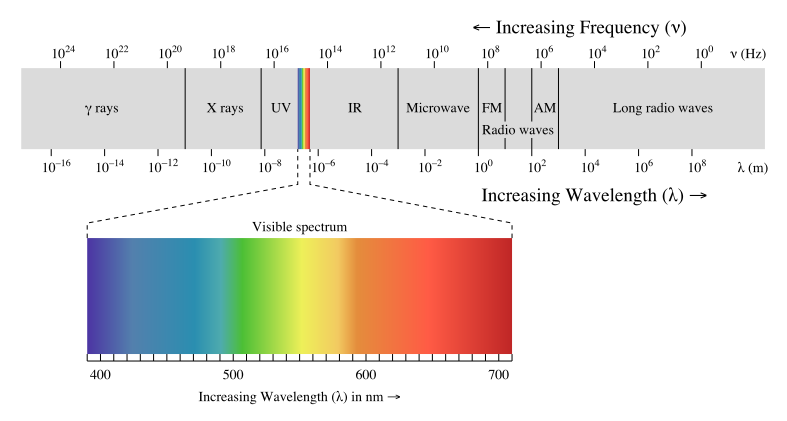
\includegraphics[width=\textwidth]{emSpectrum.pdf}
\end{figure}
\end{frame}


%----------------------------------------------------------------------------------------

\subsection*{Gamma-ray imaging}

%----------------------------------------------------------------------------------------

\begin{frame}
Examples of gamma-ray imaging:
\begin{itemize}
\item Nuclear medicine. Patient take radioactive isotopes.
\item Astronomy.
\end{itemize}
\begin{figure}
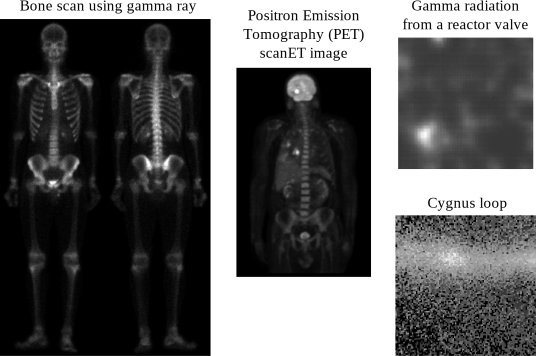
\includegraphics[width=\textwidth]{gammaRayImaging.pdf}
\end{figure}
\end{frame}

%----------------------------------------------------------------------------------------

\subsection*{X-ray imaging}

%----------------------------------------------------------------------------------------

\begin{frame}
X-ray imaging:
\begin{itemize}
\item Medicine.
\begin{itemize}
\item Radiography.
\item Angiography (Contrast Enhancement Radiography).
\item Computerized Axial Tomography (CAT).
\end{itemize}
\end{itemize}
\begin{figure}
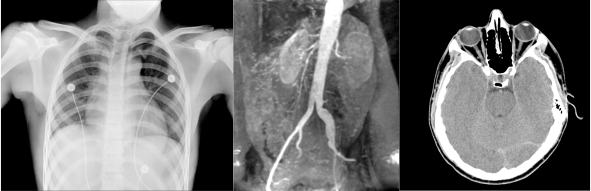
\includegraphics[width=\textwidth]{xRayImaging-medicine.png}
\end{figure}
\end{frame}

%----------------------------------------------------------------------------------------

\begin{frame}
X-ray imaging:
\begin{itemize}
\item Industry:
\begin{itemize}
\item Flaw detection.
\end{itemize}
\end{itemize}
\begin{figure}
\includegraphics[width=.5\textwidth, angle=90]{Fig1_07(d).jpg}
\end{figure}
\end{frame}

%----------------------------------------------------------------------------------------

\subsection*{Ultra-Violet (UV) imaging}

%----------------------------------------------------------------------------------------

\begin{frame}
Ultra-violet (UV) imaging:
\begin{itemize}
\item Fluorescence microscopy.
\end{itemize}
\begin{figure}
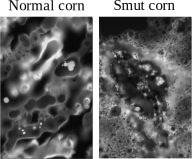
\includegraphics[scale=1]{UVimaging.pdf}
\end{figure}
\end{frame}

%----------------------------------------------------------------------------------------

\subsection*{Visible and infrared imaging}

%----------------------------------------------------------------------------------------

\begin{frame}
Visible and infrared imaging.
\begin{itemize}
\item Light microscopy.
\item Astronomy.
\item Remote sensing.
\item Industry.
\item Law enforcement.
\end{itemize}
\end{frame}

%----------------------------------------------------------------------------------------

\begin{frame}
\begin{columns}
\begin{column}{.48\textwidth}
Light microscopy imaging:
\begin{itemize}
\item Anti-cancer agent -- 250$\times$.
\item Cholesterol -- 40$\times$.
\item Microprocessor -- 60$\times$.
\end{itemize}
\end{column}
\begin{column}{.48\textwidth}
\begin{figure}
\includegraphics[width=1.3\textwidth,angle=-90]{lightMicroscopy1.png}
\end{figure}
\end{column}
\end{columns}
\end{frame}

%----------------------------------------------------------------------------------------

\begin{frame}
\begin{columns}
\begin{column}{.48\textwidth}
Light microscopy imaging:
\begin{itemize}
\item Nikel-oxide thin film -- 600$\times$.
\item Audio CD surface -- 1750$\times$.
\item Organic superconductor -- 450$\times$.
\end{itemize}
\end{column}
\begin{column}{.48\textwidth}
\begin{figure}
\includegraphics[width=1.3\textwidth,angle=-90]{lightMicroscopy2.png}
\end{figure}
\end{column}
\end{columns}
\end{frame}

%----------------------------------------------------------------------------------------

\begin{frame}
Remote sensing.
\begin{itemize}
\item Environmental monitoring.
\item Population growth assessment, land occupation.
\item Hazard prediction.
\end{itemize}
\end{frame}

%----------------------------------------------------------------------------------------

\begin{frame}
Remote sensing.
\begin{figure}
\includegraphics[width=\textwidth]{remoteSensingImaging0.png}
\end{figure}
\end{frame}

%----------------------------------------------------------------------------------------

\begin{frame}
Remote sensing.
\begin{figure}
\includegraphics[width=\textwidth]{remoteSensingImaging.png}
\end{figure}
\end{frame}

%----------------------------------------------------------------------------------------

\begin{frame}
Industry.
\begin{figure}
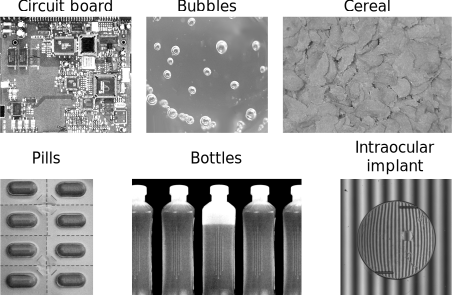
\includegraphics[width=\textwidth]{visualIndustrialInspection.pdf}
\end{figure}
\end{frame}

%----------------------------------------------------------------------------------------

\begin{frame}
Law-enforcement.
\begin{figure}
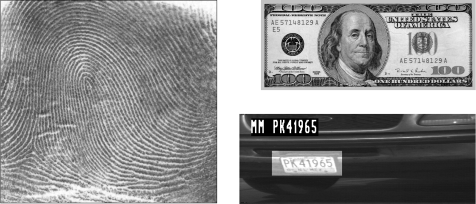
\includegraphics[width=\textwidth]{visualIndustrialInspection2.png}
\end{figure}
\end{frame}

%----------------------------------------------------------------------------------------

\subsection{Microwave band}

%----------------------------------------------------------------------------------------

\begin{frame}
Radar.
\begin{itemize}
\item Insensitive to weather conditions.
\item Microwave energy reflected back is registered as image.
\item Example: south Tibet mountains:
\end{itemize}
\begin{figure}
\includegraphics[width=.7\textwidth]{radar.jpg}
\end{figure}
\end{frame}

%----------------------------------------------------------------------------------------

\subsection{Radio band imaging}

%----------------------------------------------------------------------------------------

\begin{frame}
Medicine.
\begin{itemize}
\item Magnetic Resonance Imaging (MRI).
\item Radio waves stimulates responses from the tissues.
\end{itemize}
\begin{columns}
\begin{column}{.48\textwidth}
Knee.
\begin{figure}
\includegraphics[width=\textwidth]{MRIKnee.jpg}
\end{figure}
\end{column}
\begin{column}{.48\textwidth}
Spine.
\begin{figure}
\includegraphics[width=\textwidth]{MRISpine.jpg}
\end{figure}
\end{column}
\end{columns}
\end{frame}

%----------------------------------------------------------------------------------------

\subsection{Other imaging modalities}

%----------------------------------------------------------------------------------------

\begin{frame}
Acoustic imaging.
\begin{itemize}
\item Geological (mineral and oil) exploration.
\begin{itemize}
\item Low end (hundreds of Hz).
\item Ultrasound (millions of Hz).
\end{itemize}
\item Industry.
\item Medicine.
\begin{itemize}
\item Imaging unborn babies.
\end{itemize}
\end{itemize}
\end{frame}

%----------------------------------------------------------------------------------------

\begin{frame}
Acoustic imaging.
\begin{enumerate}
\item The ultrasound system (a computer, ultrsound probe consisting of a source, a receive, and a display) transmits high-frequency (1 to 5 MHz) sound pulses into the body.
\item The sound waves travel into the body and hit a boundary between tissues (e.g., between fluid and soft tissue, soft tissue and bone). Some of the sound waves are reflected back to the probe, while some travel on further until they reach another boundary and are reflected.
\item The reflected waves are picke up by the probe and relayed to the computer.
\item The machine calculates the distance from the probe to the tissue or organ boundaries using the speed of sound in tissue (1540 m/s) and the time of each echo's return.
\item The system displays the distances and intensities of the echoes on the screen, forming a two-dimensional image.
\end{enumerate}
\end{frame}

%----------------------------------------------------------------------------------------

\begin{frame}
\begin{figure}
\includegraphics[width=.8\textwidth]{baby.jpg}
\end{figure}
\end{frame}

%----------------------------------------------------------------------------------------

\begin{frame}
Acoustic imaging.
\begin{figure}
\includegraphics[width=\textwidth]{seismic}
\caption{Cross-sectional image of a seismic model. The arrow points to a hydrocarbon (oil and/or gas) trap. (Courtesy of Dr. Curtis Ober, Sandia National Laboratories).}
\end{figure}
\end{frame}

%----------------------------------------------------------------------------------------

\begin{frame}
\begin{itemize}
\item Electron microscopy
\begin{itemize}
\item Can achieve 10.000$\times$ magnification or more (Optical = up to $1000\times$).
\item Uses a focused beam of electrons instead of light.
\item Scanning Electron Microscope (SEM):
\end{itemize}
\end{itemize}
\begin{columns}
\begin{column}{.48\textwidth}
\begin{figure}
\includegraphics[width=.7\textwidth]{thermalFailure-a.jpg}
\caption{250$\times$ image of tungsten filament with thermal failure.}
\end{figure}
\end{column}
\begin{column}{.48\textwidth}
\begin{figure}
\includegraphics[width=.9\textwidth]{thermalFailure-b.jpg}
\caption{2500$\times$ image of damaged integrated circuit.}
\end{figure}
\end{column}
\end{columns}
\end{frame}

%----------------------------------------------------------------------------------------

\begin{frame}
Synthetic (computer-generated) images.
\begin{itemize}
\item Fractals.
\begin{itemize}
\item Iterative reproduction of a basic pattern according to some mathematical rules.
\item Useful sometimes as random textures.
\end{itemize}
\item 3-D modeling.
\begin{itemize}
\item 3-D model projects a synthetic image.
\item Flight simulation.
\item Medical training.
\item Criminal forensics.
\item Special effects.
\end{itemize}
\end{itemize}
\end{frame}

%----------------------------------------------------------------------------------------

\section{Overview of DIP}

%----------------------------------------------------------------------------------------

\begin{frame}
\begin{figure}
\includegraphics[width=\textwidth]{overviewDIP.png}
\end{figure}
\end{frame}

%----------------------------------------------------------------------------------------

\section{General components of a DIP system}

%----------------------------------------------------------------------------------------

\begin{frame}
\begin{figure}
\includegraphics[width=.7\textwidth]{components.png}
\end{figure}
\end{frame}



%%----------------------------------------------------------------------------------------
%%----------------------------------------------------------------------------------------
%%----------------------------------------------------------------------------------------
%%----------------------------------------------------------------------------------------
%%----------------------------------------------------------------------------------------
%
%\subsection{Background}
%
%\begin{frame}
%Use the following to solve problems:
%\begin{itemize}[<+->]
%\item Theoretical base.
%\item State-of-the-art software (MATLAB).
%\item High level of experimentation.
%\end{itemize}
%\end{frame}
%
%\begin{frame}
%Ability to:
%\begin{itemize}
%\item Formulate approaches.
%\item Quickly prototype candidate solutions.
%\end{itemize}
%\end{frame}
%
%\begin{frame}
%We’re interested in the:
%Bridge the gap between theory and application.
%\end{frame}
%
%
%Leading theoretical book:
%Gonzalez \& Woods, "Digital Image Processing”. Prentice Hall.
%Leading software package:
%MATLAB® \textit{Image Processing Toolbox} (IPT).
%
%Examples ranging between
%Medicine
%Industrial inspection
%Remote sensing
%Astronomy
%
%MATLAB
%
%%----------------------------------------------------------------------------------------
%
%\subsection{What is Digital Image Processing?}
%
%%----------------------------------------------------------------------------------------
%
%\begin{frame}
%\begin{itemize}[<+->]
%\item An image is a two dimensional function $f(x,y)$ containing intensities.
%\item If $x$, $y$ and $f(x,y)$ are discrete $\rightarrow$ digital image.
%\item A digital image is composed of a finite number of elements called ``\textbf{P}icture \textbf{EL}ements'' (PELs), \textit{pixels}, \textit{image elements}.
%\end{itemize}
%\end{frame}
%
%%----------------------------------------------------------------------------------------
%
%\section{The human vision}
%
%%----------------------------------------------------------------------------------------
%
%\begin{frame}
%\begin{itemize}
%\item Vision is the most advanced of human senses.
%\item But humans see only a small portion of the electromagnetic spectrum.
%\item But machines see beyond:
%\begin{itemize}
%\item Gamma and radio waves.
%\end{itemize}
%\item Also using different sources:
%\begin{itemize}
%\item Ultrasound.
%\item Electron microscopy.
%\item Computer generated images.
%\end{itemize}
%\end{itemize}
%\end{frame}
%
%%----------------------------------------------------------------------------------------
%
%\begin{frame}
%Paradigm according to computational processing:
%\begin{itemize}
%\item Low-level (both input and output are images): primitive operations, such as:
%\begin{itemize}
%\item Image pre-processing to reduce noise.
%\item Contrast enhancement.
%\item Image sharpening.
%\end{itemize}
%\item Mid-level:
%\begin{itemize}
%\item Inputs: images.
%\item Outputs: attributes.
%\end{itemize}
%\end{itemize}
%\end{frame}
%
%%----------------------------------------------------------------------------------------
%
%\begin{frame}
%Paradigm according to computational processing:
%\begin{itemize}
%\item High-level:
%\begin{itemize}
%\item Image understanding.
%\item Extract sense from an ensemble of elements.
%\item Computer vision.
%\end{itemize}
%\end{itemize}
%\end{frame}

%----------------------------------------------------------------------------------------

\section{Development tools}

%----------------------------------------------------------------------------------------

\begin{frame}
\begin{columns}
\begin{column}{.5\textwidth}
Development tools:
\begin{itemize}
\item \href{http://www.mathworks.com/products/matlab/}{Matlab$^{\textregistered}$} (octave - GNU).
\item \href{http://opencv.org/}{OpenCV}.
\item \href{http://imagej.nih.gov/ij/}{ImageJ}.
\item \href{http://www.photoshop.com/}{Photoshop}.
\item \href{http://www.gimp.org/}{Gimp}.
\item \href{https://inkscape.org/en/}{Inkscape}.
\item \href{https://docs.anaconda.com/anaconda/navigator/}{Anaconda-navigator}
\end{itemize}
\end{column}
\begin{column}{.5\textwidth}
\begin{figure}

\includegraphics[width=\textwidth]{logos.png}
\end{figure}
\end{column}
\end{columns}
\end{frame}

%----------------------------------------------------------------------------------------

\subsection{MATLAB}

%----------------------------------------------------------------------------------------

\begin{frame}
What is MATLAB$^{\textregistered}$?
\begin{itemize}
\item High-performance language for technical computing.
\item Matrix Laboratory.
\item Integrates:
\begin{itemize}
\item Computation.
\item Visualization.
\item Programming.
\end{itemize}
\item Easy to use environment.
\end{itemize}
\end{frame}

%----------------------------------------------------------------------------------------

\begin{frame}
Typical uses:
\begin{itemize}
\item Math and computation.
\item Algorithm development.
\item Data acquisition.
\item Scientific and engineering graphics.
\item Application development (GUI).
\end{itemize}
\end{frame}

%----------------------------------------------------------------------------------------

\begin{frame}
MATLAB is widely used in Universities:
\begin{itemize}
\item Math, engineering, science.
\end{itemize}
Industries:
\begin{itemize}
\item Research, development and analysis.
\end{itemize}
\end{frame}

%----------------------------------------------------------------------------------------

\begin{frame}
\textit{Toolboxes}:
\begin{itemize}
\item Collection of application-specific functions (\textit{M-functions} or \textit{M-files}).
\item Extend the core capabilities of MATLAB.
\end{itemize}
Examples:
\begin{itemize}
\item Image Processing Toolbox (IPT).
\item Signal Processing Toolbox.
\item Neural Network.
\item Fuzzy Logic.
\item Wavelet.
\end{itemize}
\end{frame}

%----------------------------------------------------------------------------------------

\subsection{OpenCV}

%----------------------------------------------------------------------------------------

\begin{frame}
OpenCV (Open Source Computer Vision Library).
\begin{itemize}
\item Initially developed by Intel.
\item Free for both academic and commercial use.
\item C++, C, Python and Java interfaces.
\item Multi-core processing.
\item OpenCL -- hardware acceleration of the underlying compute platform.
\end{itemize}
\end{frame}

%----------------------------------------------------------------------------------------

\begin{frame}
Applications:
\begin{itemize}
\item Street view image stitching.
\item Automated inspection and surveillance.
\item Robot and driver-less car navigation and control.
\item Medical image analysis.
\item Video/image search and retrieval.
\item Movies - 3D structure from motion.
\item Interactive art installations.
\end{itemize}
\end{frame}

%----------------------------------------------------------------------------------------

\begin{frame}
Functionality:
\begin{enumerate}
\item Image/video I/O (core).
\item Processing (imgproc).
\item Display (highgui).
\item Object/feature detection (objdetect, features2d, nonfree).
\end{enumerate}
\end{frame}

%----------------------------------------------------------------------------------------

\begin{frame}
Functionality:
\begin{enumerate}
\setcounter{enumi}{4}
\item Geometry-based monocular or stereo computer vision (calib3d, stitching, videostab).
\item Computational photography (photo, video, superres).
\item Machine learning \& clustering (ml, flann)
\item CUDA  acceleration (gpu).
\end{enumerate}
\end{frame}

%----------------------------------------------------------------------------------------

\subsection{Auxiliary tools}

%----------------------------------------------------------------------------------------

\begin{frame}
Useful tools for prototyping.
\begin{itemize}
\item ImageJ.
\item GIMP.
\item Photoshop.
\end{itemize}
\end{frame}

%----------------------------------------------------------------------------------------

\section{References}

%----------------------------------------------------------------------------------------

\begin{frame}
\frametitle{References}
\footnotesize{
\begin{thebibliography}{99} % Beamer does not support BibTeX so references must be inserted manually as below
\bibitem[Gonzalez2012]{p1} Gonzalez, Rafael C.; Woods, Richard E. (2018)
\newblock Digital Image Processing
\newblock \emph{Pearson} 4$^{th}$ Ed..
%
\bibitem[Gonzalez2009]{p1} Gonzalez, Rafael C.; Woods, Richard E. (2009)
\newblock Digital Image Processing Using Matlab
\newblock \emph{Pearson} 2$^{nd}$ Ed..
\end{thebibliography}
}
\end{frame}
%
%material presented
%
%Gonzalez, Rafael C.; Woods, Richard E. (2012-06-20). Digital Image Processing (3rd Edition) (Page 31). Pearson HE, Inc.. Kindle Edition. 
%----------------------------------------------------------------------------------------

%\begin{frame}
%\frametitle{Referências}
%\footnotesize{
%\begin{thebibliography}{99} % Beamer does not support BibTeX so references must be inserted manually as below
%\bibitem[Oliveira, 2013]{p1} Oliveira, H. M. (2013)
%\newblock Engenharia de Telecomunicações
%\newblock \emph{Ed. UFPE} 2$^{a}$ Ed..
%%
%\bibitem[Haykin, 2007]{p1} Haykin, S., e Moher, M. (2007)
%\newblock Introduction to Analog and Digital Communications
%\newblock \emph{Ed. Wiley} 2$^{a}$ Ed..
%\end{thebibliography}
%}
%\end{frame}

%\bibliographystyle{IEEEtran}
% argument is your BibTeX string definitions and bibliography database(s)
%\bibliography{biblio}
%----------------------------------------------------------------------------------------

\end{document} 
